\documentclass[a4paper,12pt]{article}

%A Few Useful Packages
\usepackage{marvosym}
\usepackage{fontspec} 					%for loading fonts
\usepackage{xunicode,xltxtra,url,parskip} 	%other packages for formatting
\RequirePackage{color,graphicx}
\usepackage[usenames,dvipsnames]{xcolor}
\usepackage[big]{layaureo} 				%better formatting of the A4 page
% an alternative to Layaureo can be ** \usepackage{fullpage} **
\usepackage{supertabular} 				%for Grades
\usepackage{titlesec}					%custom \section
\usepackage{array}

%Setup hyperref package, and colours for links
\usepackage{hyperref}
\definecolor{linkcolour}{rgb}{0,0.2,0.6}
\hypersetup{colorlinks,breaklinks,urlcolor=linkcolour, linkcolor=linkcolour}

%FONTS
\defaultfontfeatures{Mapping=tex-text}
%\setmainfont[SmallCapsFont = Fontin SmallCaps]{Fontin}
%%% modified for Karol Kozioł for ShareLaTeX use
\setmainfont[
SmallCapsFont = Fontin-SmallCaps.otf,
BoldFont = Fontin-Bold.otf,
ItalicFont = Fontin-Italic.otf
]
{Fontin.otf}
%%%

%CV Sections inspired by: 
%http://stefano.italians.nl/archives/26
\titleformat{\section}{\Large\scshape\raggedright}{}{0em}{}[\titlerule]
\titlespacing{\section}{0pt}{3pt}{3pt}
%Tweak a bit the top margin
%\addtolength{\voffset}{-1.3cm}

% Adding tabs and itemuze to tabular
\usepackage{booktabs}% http://ctan.org/pkg/booktabs
\newcommand{\tabitem}{~~\llap{\textbullet}~~}

%Italian hyphenation for the word: ''corporations''
\hyphenation{im-pre-se}

%-------------WATERMARK TEST [**not part of a CV**]---------------
\usepackage[absolute]{textpos}

\setlength{\TPHorizModule}{30mm}
\setlength{\TPVertModule}{\TPHorizModule}
\textblockorigin{2mm}{0.65\paperheight}
\setlength{\parindent}{0pt}

% Adding if execution to define between thesis and article
\usepackage{ifthen}
\newboolean{CV} % Is it a resule or CV
\setboolean{CV}{true}
\newboolean{SE} % Is in an IT CV or a Software Engineers
\setboolean{SE}{true}

% Add PDF
\usepackage[final]{pdfpages}
%--------------------BEGIN DOCUMENT----------------------
\begin{document}

%WATERMARK TEST [**not part of a CV**]---------------
%\font\wm=''Baskerville:color=787878'' at 8pt
%\font\wmweb=''Baskerville:color=FF1493'' at 8pt
%{\wm 
%	\begin{textblock}{1}(0,0)
%		\rotatebox{-90}{\parbox{500mm}{
%			Typeset by Alessandro Plasmati with \XeTeX\  \today\ for 
%			{\wmweb \href{http://www.aleplasmati.comuv.com}{aleplasmati.comuv.com}}
%		}
%	}
%	\end{textblock}
%}

\pagestyle{empty} % non-numbered pages

\font\fb=''[cmr10]'' %for use with \LaTeX command

%--------------------TITLE-------------
\par{\centering
		{\Huge Marat (Matt) \textsc{Sadykov}
	}\bigskip\par}

%--------------------SECTIONS-----------------------------------
%Section: Personal Data
\section{Personal Information}

\begin{tabular}{rl}
    %\textsc{Address:}   & 3/22 Prince Street, Gaythorne, Brisbane, QLD, 4051 \\
    \textsc{Address:}   & Brisbane, Queensland, Australia\\
    \textsc{Phone:}     & +61 478 686 650\\
    \textsc{Email:}     & \href{mailto:sadykovmarat@pm.me}{sadykovmarat@pm.me} \\
    \textsc{LinkedIn:}  & \href{https://www.linkedin.com/in/marat-sadykov-0a93b0133/}{marat-sadykov-0a93b0133} \\
    \textsc{GitHub:}    & \href{https://github.com/SmugglerSMR}{SadykovMR Profile} \\
    \textsc{ORCID:}    & \href{https://orcid.org/0000-0002-6436-7069}{0000-0002-6436-7069} \\
    \textsc{Work rights:} & \href{https://immi.homeaffairs.gov.au/visas/getting-a-visa/visa-listing/student-500}{Bridge VISA after Postgraduate Research (subclass 500)} -> \\
    & \href{https://immi.homeaffairs.gov.au/visas/getting-a-visa/visa-listing/temporary-graduate-485/post-study-work}{Post-Study Work (subclass 485) VISA} (2-4 years)
    %\\ & (Ended on: 18-Jan-2024) 
    % \textsc{Stack Overflow:}    & \href{https://stackoverflow.com/users/8673205/smuggler}{smuggler Profile}
\end{tabular}

%Section: Education
\section{Education and Training}
\begin{tabular}{rl}	
    \textsc{Sept} 2019-2023 & \hyperref[magister]{\textbf{Master of Philosophy}}, school of \\ 
    % \textsc{Sept} 2019-2022 & \textbf{Master of Philosophy}, school of \\
                            & \textsc{Mechanical Medical \& Process Engineering}, \\ 
                        & \textbf{Queensland University of Technology}, Brisbane \\
    %Time-Series Machine Learning in Electrical Vehicles: Smart Battery Management through Neural-Network-Based State of Charge Prediction
    & \small\emph{Thesis Topic}: Time-Series Machine Learning in Electrical Vehicles: Smart \\
    & \small \ \ \ \ \ \ \ \ \ \ \ \ \ \ \ \ \ \ \ Battery Management through Neural-Network-Based State \\
    & \small \ \ \ \ \ \ \ \ \ \ \ \ \ \ \ \ \ \ \ of Charge Prediction \\
    & \small \ \ \ \ \ \ \ \ \ \ \ \ \ \ \ \ \ \ \ Financed by Automotive Engineering Graduate Program (AEGP)\\ 
    & \small \ \ \ \ \ \ \ \ \ \ \ \ \ \ \ \ \ \ \ in cooperation with Prohelion as an industry partner \\
    % IF
    \ifthenelse {\boolean{SE}}
    %
    % THEN
    {
   & \small\emph{Primary Area:}  Large sensor data processing to create multiple parallel State of\\
   & \small \ \ \ \ \ \ \ \ \ \ \ \ \ \ \ \ \ \ \ \ Charge Machine Learning models using High-Performance Computing \\
    %& \small\emph{Primary Area} : Embedded Software Developer of Time-Series Machine  \\
    %& \small \ \ \ \ \ \ \ \ \ \ \ \ \ \ \ \ \ \ \ \ \ learning (ML) model for Electric Vehicles \\
    & \small\emph{$2^{nd}$ Area:} Application of Machine Learning in Low-power Embedded devices, such \\
    & \small \ \ \ \ \ \ \ \ \ \ \ \ \ \ as Android, Raspberry Pi boards and TPU-enhanced controllers \\
    % & \small\emph{3ry Area} : Medical engineering and ML application for body/brain conditions \\
    } {}
% 	\textit{Expected completion date}: August 2021
    &\normalsize \textsc{Level 9 Qualification} \\
% 	&\\
%%%%%%%%%%%%%%%%%%%%%%%%%%%%%
	\textsc{July} 2015-2019 & \hyperref[bachelor]{\textbf{Bachelor of Engineering (Honours)}}, major in \\
	& \textsc{Computer and Software Systems (CSS)}, \\
	& Second Major: \textsc{Computational and Simulation Science} \\ 
	& \textbf{Queensland University of Technology}, Brisbane \\ 
	& \small\emph{Primary Engineering Disciplines:} Telecommunications \& Control and Dynamics\\
	& \small\emph{Primary Software Area:} High and Low Level Development \& \\
	& \small \ \ \ \ \ \ \ \ \ \ \ \ \ \ \ \ \ \ \ \ \ \ \ \ \ \ \ \ \ \ \ \ \ \ Cloud and parallel High Performance Computing (HPC) \\ 
	% IF
    \ifthenelse {\boolean{SE}}
    %
    % THEN
    {
	& \small\emph{$2^{nd}$  Major:} Large Data-set Visualisation \& Machine Learning\\ 
	& \small\emph{Honours Research Topic:} Tank Commander Mixed Reality Simulation using \\
	& \small \ \ \ \ \ \ \ \ \ \ \ \ \ \ \ \ \ \ \ \ \ \ \ \ \ \ \ \ \ \ \ \ \ \ \ \ Unity Game Engine and TensorFlow \\
	} {}
	%& \textit{Expected completion date}: June 2019 \\
	&\normalsize \textsc{GPA:} 6.1/7.0 \\
	%\hyperlink{grds}{\hfill | \footnotesize Detailed List of Exams}
% 	&\\
%%%%%%%%%%%%%%%%%%%%%%%%%%%%%
	2014 - 2015& Standard Foundation in \textbf{Foundation Standard to Degree Pathway} \\&\normalsize\textbf{Queensland University of Technology for International Students} \\ &\normalsize \textsc{GPA:} 6.3/7.0 %\hyperlink{grds_cleli}{\hfill| \footnotesize Detailed List of Exams}
% 	\\&\\
\end{tabular}

\section{Key Technical Skills}
\begin{tabular}{rl}
	Developed skills & \small\emph{Primary Languages} : \textsc{C} and \textsc{Python} \\
	& \small\emph{Secondary Languages} : \textsc{C++},\textsc{C\#}, \textsc{Java}, \textsc{JavaScript} \\
	& \small\emph{Tertiary Languages} : \textsc{F\#}, \textsc{R}, \textsc{Rust}, \textsc{Julia}, \textsc{SQL}, \textsc{Swift}, \textsc{Assembler} \\
	Additional skills & \small {\fb \LaTeX}\setmainfont[SmallCapsFont=Fontin-SmallCaps.otf]{Fontin.otf}, GIT, MATLAB, ParaView, IntelliJ, Code Composer Studio, RTOS, \\
	\& \small environments : & STM32CubeMX/TrueStudio, Cython, C to Python wrappers, Conda, \\
	& \small Numpy \& Pandas, PyTests, TensorFlow, AWS, Flask, CUDA, Unity Game Engine, \\
	& \small ClickHouse-driver \\ 
	% IF
    \ifthenelse {\boolean{CV}}
    %
    % THEN
    {
    & Hyper-virtualisation, Para-virtualisation and Nested-virtualisation \\
    & using devices pass-through with QEMU/KVM and Xen \\ \\
% 	Operational & Windows (CE, 98, 2003 server, XP, 7, 8, 8.1, 10), \\
	Operational & Windows, Macintosh, Berkeley Software Distribution (BSD), \\ 
	Systems (OS) & Linux (Debian-based: Ubuntu 14.04 and higher, \\
	& \ \ \ \ \ \ \ \ \ \ RedHat-based: RHEL8, Fedora-32 and higher), \\ 
% 	& Mac OS X (Maverick, Sierra and higher), Android (4.0.4 and higher). \\
% 	& Unix-Like (FreeBSD, GhostBSD) \\
        % IF
        \ifthenelse {\boolean{SE}}
        %
        % THEN
        {
	Owner of: & Australian Blue Card, Car Driving Open License 
	    }{}
	}
	{
	} \\ [1pc]
	
\end{tabular} \\[1pc]
% IF
\ifthenelse {\boolean{CV}}
%
% THEN
{
    % IF
    \ifthenelse {\boolean{SE}}
    %
    % THEN
    {
\textbf{Developed understanding in a variety of Algorithms (Searching and Sorting), Machine Learning using TensorFlow (Implemented a large functional library of useful methods C code wrappers to Python to increase performance during research, involving optimisation and parallel multi-GPU computation),
and Cloud programming with AWS for data storage and processing.
Mastered common known operational systems (OSs) through Xen and QEMU/KVM para and nested virtualisation.}
    } {}
} {}

%Section: Languages
%
% IF
\ifthenelse {\boolean{CV}}
%
% THEN
{
    % IF
    \ifthenelse {\boolean{SE}}
    %
    % THEN
    {
\section{Scholarships and Certificates}
\begin{tabular}{rl}
 \textsc{Sept} 2021 & QUT Write-Up scholarship to complete additional publication. \\
 \textsc{Aug} 2021 & (e-Grad School) Transdisciplinarity in Research. \\
 \textsc{Mar} 2021 & (Surf Life Saving) First-Aid Training. \\
 \textsc{June} 2020 & 
 \href{https://business.gov.au/grants-and-programs/automotive-engineering-graduate-program/aegp-grant-recipients}{Automotive Engineering Graduate Program (AEGP)} for Intelligent \\
 & BMS for large cell format Lithium Ion battery storage systems in \\
 & electric vehicles \footnotesize(\$ 284,275)\normalsize\\
 
%  
\end{tabular}
    } {}
\section{Languages}
    % IF
    \ifthenelse {\boolean{SE}}
    %
    % THEN
    {
\begin{tabular}{rl}
	\textsc{Russian:} &Mother tongue. 
	% Lived and worked in Russia as private technical support.\\ 
	Born and studied there for 11 years and finished High school \\ 
	& with Honour, Gold Medal and Red Certificate. \\ [1pc]
	\textsc{English:} &Fluent. Received high and research degree education in Brisbane, Australia. \\
	%& after completing secondary education in Russia.\\
	& IELTS score (7.5/9.0) - L:9.0, R:7.5, W:6.5 S:7.5
\end{tabular}
    }
    {
\begin{tabular}{rl}
	\textsc{Russian:} & Mother tongue. \\
	\textsc{English:} &Fluent. IELTS score (7.5/9.0) - L:9.0, R:7.5, W:6.5 S:7.5
\end{tabular}
    }
    % IF
    \ifthenelse {\boolean{SE}}
    %
    % THEN
    {
\section{Publications}
\begin{tabular}{rl}
%  \textsc{Octo} 2021 & (In Progress) Real Time SoC estimation using Machine Learning\\
%  & on embedded devices from Electric Vehicle and Bi-directional power supplier\\
%  & accumulator cycling data. \\
 \textsc{Nov} 2022 & (Under review) Feed-Forward State of Charge estimation using Time-Series \\
 & With Autoregressive Models. Journal of Power Sources. \\
 \textsc{Dec} 2022 & Sadykov, Marat, Sam Haines, Mark Broadmeadow, Geoff Walker, \\
 & and David William Holmes. 2023. "Practical Evaluation of Lithium-Ion \\
 & Battery State-of-Charge Estimation Using Time-Series Machine Learning \\
 & for Electric Vehicles" Energies 16, no. 4: 1628. \href{https://doi.org/10.3390/en16041628}{https://doi.org/10.3390/en16041628}
\end{tabular}
    } {}
}
{}
%Section: Work Experience at the top
\section{Employment History}
\begin{tabular}{r|p{11cm}}
    % Final year research
    \emph{Dec 2020} &Tutor for Systems Programming, Software Development and Advanced Systems Design Units \textsc{QUT} \\\textsc{Feb 2020}&\emph{Sessional Academic tutor for university units.}\\&\footnotesize{Developing students' low-level C programming techniques, high-level Java Software Development and writing and supervising semester-wide projects, which combines all the above skills to develop final year projects using TensorFlow and Python for Image Processing, Gas Sensor readings and Web-based server deployment.}\\\multicolumn{2}{c}{} \\ [1pc]
	
	\emph{May 2019} & Software Developer on a Laravel-based project at \textsc{NetComp} \\\textsc{Feb 2018}&\emph{Software Developer.}\\&\footnotesize{The company's project is based on PHP, JavaScript, and Laravel, which are established in AWS. The project was distributed across several client companies. The job was to improve, design and implement new architecture, preserving and further maintaining client data.}\\\multicolumn{2}{c}{} \\ [1pc]
	
	\emph{Dec 2019} &Tutor for Software Development Unit \textsc{QUT} \\\textsc{Feb 2018}&\emph{Sessional Academic tutor for university unit.}\\&\footnotesize{Developing students' high-level programming knowledge using Java, Agile practices, version control with Git, and test-driven development.}\\\multicolumn{2}{c}{} \\ [1pc]
	
	\emph{Dec 2018} &Tutor for Systems Programming and Microprocessors and Digital Systems Units \textsc{QUT} \\\textsc{Jul 2018}&\emph{Sessional Academic tutor for university units.}\\&\footnotesize{Developing students' low-level C programming techniques for First and Fourth-year students.}\\\multicolumn{2}{c}{} \\ [1pc]
	
	\emph{Feb 2018} & Software Engineering Intern at \textsc{Deeep Sense} \\\textsc{Nov 2017}&\emph{Developing Android App with NFC communication.}\\&\footnotesize{Implemented an application for a quick Near Field Communication (NFC) file transfer. This approach will be used to save buying receipts straight to a smartphone instead of a printed copy or email message.}\\\multicolumn{2}{c}{}
% \ifthenelse{\boolean{CV}}
% {
%     \ifthenelse {\boolean{SE}}
%     {
%     \\ [1pc]
% 	\emph{Feb 2018} & Virtual Reality Research for Kitchen Simulation as \textsc{QUT VRES} - (Vocation Research Project) \\\textsc{Nov 2017}&\emph{VR Programmer}\\&\footnotesize{Implemented a virtual avatar as a companion who will guide and track user activities around established area. This is Vocation Research Project at QUT, supervised by Dr Ross Brown.}\\\multicolumn{2}{c}{} \\ [1pc]
% 	} {}
% }{
% }
%%%%%%%%%%%%
\end{tabular}
% \newpage
%     \ifthenelse {\boolean{SE}}
%         {
% \begin{tabular}{r|p{11cm}}
%     \emph{Nov 2017} & Software Developer at \textsc{MultiCap} \\\textsc{Aug 2017}&\emph{Python VI Programmer}\\&\footnotesize{Implemented small VI for company robot to interact with children. Discovered ways to recognise faces, object and voices. Established interaction to fir physiologists' needs.}\\\multicolumn{2}{c}{}  \\	[1pc]
 
% 	\textsc{Mar 2017} & Freelancer Project.\textsc{Web Browser Extension} \\\textsc{Feb 2017}&\emph{FFmpeg for WinRT Extension}\\&\footnotesize{Configure Open Source \textit{FFmpeg} to be integrated to \textit{WinRT} Extension to fit new Windows 10 settings. Using limited sources and communications with Microsoft Technical support team, achieved purpose for continues work.}\\\multicolumn{2}{c}{} \\ [1pc]
% 	%%%%%%%%%%%%%
% 	\textsc{2015-2017} & Freelances Job, \emph{Test Development and Personal Project}\\&\footnotesize{Primary job as Test Developer for Web Pages, databases and Extensions. Most of the time using \textit{Selenium}. Simultaneously, developing personal project for Google Chrome \textit{Native Client} Video and Audio Converter using Open Source \textit{FFmpeg}.}	
% \end{tabular}
%     } {}
\ifthenelse{\boolean{CV}}
{
    % IF
    \ifthenelse {\boolean{SE}}
    %
    % THEN
    {
\section{University Activity}
	\begin{tabular}{rl}
		\textsc{2020-2021} & Partnered with QUT Motorsport guild due to research requirements. \\	
		\textsc{2020} & Become a leading tutor for the Advanced System Design university unit. \\	
%		\textsc{2017} & Become active member of \textbf{CODE Network} university society. \\
		\textsc{2018-2019} & Became a QUT Tutor for High and Low level programming units. \\
		\textsc{2017} & Participated in QUT Engineering filming video. \\
		\textsc{2018} & Received QUT Dean's List for Excellent Academic Performance \\
		\textsc{2017} & QUT Peer Career Ambassador Volunteer \\ 
		    & \tabitem 20 and 22 hours over Semester 1 and 2. \\
		\textsc{2016} & Member of the Golden Key International Honour Society \\&– for students with a GPA above 6. %\footnote{Here presented most recent and relevant experience}
	\end{tabular}
	} {}
}
{}
%Section: Scholarships and additional info
\section{Relevant Projects and University Involvement}
% \subsection{Projects Involved}
	\begin{tabular}{rl}
	    % AEGP grant
	    \textsc{Jan} 2020 & \textbf{QUT Motorsport EV accumulator \& Battery cycling with Arbin and PSB} \\
	    & \textbf{10000 4U Bidirectional DC Power Supply.} Accumulator Battery Management \\
	    & System to measure current, voltage, and temperature to determine the State of \\
	    & Charge (SoC) as part of the Master of Philosophy research. In addition, \\
	    & research and integration embedded devices, capable of running \textbf{Machine} \\
	    & \textbf{Learning model on a low-power electric grid using TPU-accelerator} and \\
	    & Sparkfun TPU powered devices or R-pi3 w/ custom HAT CAN to Wi-Fi module. \\
	    % Machine Learning (Gaze Detection, Image Processing - Animal Detection) Cloud projects using TF-JS, Docker, Augmented Reality Final year project. Brushless Motor circuit. NFC Receipt project.
	    \textsc{Jun} 2019 & \textbf{Augmented Reality} - VR Tank Commander Simulator: \\
	        & \tabitem Reconstruction of surroundings from Kodak 360$^{\circ}$ camera to \\
	        & \textbf{Unity Game Engine}. \\ % with Raspberry Pi and Image Processing
	        & \tabitem Real-Time Image Processing with \textbf{TensorFlow} and \textbf{CUDA}. \\
	        & \tabitem \textbf{Raspberry Pi 3} controlled fully operating toy tank. \\ [1pc]
	        
        \textsc{Jun} 2019 & Embedded Systems University Project: \\
            & \tabitem Building Brushless DC motor from Texas Instruments. \\
            & \tabitem TivaC1294XL development board as primary \textbf{C} development \\
            & component and \textbf{Code Composer Studio}. \\ [1pc]
            
        \textsc{Dec} 2018 & Cloud Computing Project with Amazon Virtual Machine - \textbf{AWS}: \\
            & \tabitem Tensorlow.js to create a load on \textbf{AWS with dynamic resizing} and \\
            & detect the number of cars through webcams. \\
            & \tabitem Azure Databases to preserve the information and draw the road load \\
            & on a Google Map.\\ [1pc]
            
        \textsc{Aug} 2018 & Image Processing using Machine Learning - \textbf{TensorFlow}: \\
            & \tabitem Gaze Detection - direction of human view. \\
            & \tabitem Animal Detection - size, distance and type estimation from \\
            & bird's eye view using lenses' focal length.\\ 
            & \tabitem Landmarks detection from a flying drone using Raspberry \\
            & Pi with environmental sensors. \\ [1pc]
            
		\textsc{Jun} 2018 & Merged two \textbf{Laravel} projects to improve overall performance: \\
		    & \tabitem Combine two SQL databases by creating a Parser to simplify access. \\
		    & \tabitem Designed and built a new working environment from two old versions. \\ [1pc]
		    
		\textsc{Feb} 2018 & Developed \textbf{VR Avatar} as part of the university Vocation Research Project (VRES): \\ 
		    & \tabitem Virtual Reality companion inside Unity, guiding and tracking user activity. \\
		    & \tabitem It is intended to help people with restricted abilities to perform tasks. \\ 
		    & \tabitem Implementation of a virtual companion who will guide and track user \\ & activities around the established area.\\ [1pc]
		    
		\textsc{Jul} 2017 & Developed Computational Simulation model and Visualised with \textbf{ParaView}: \\
		    & \tabitem Supernova Remnant from a large data set. \\ [1pc]
		    
		\textsc{Mar} 2017 & Embedded Systems Design of \textbf{Digital Voice Recorder}: \\
		    & \tabitem QUT designed the Teensy board with several other components \\
		    & \tabitem Chebyshev anti-aliasing filter \textbf{LMC6484} \\ [1pc]
		    
		% \textsc{Jan} 2017 & \textbf{Developed algorithm} for video and audio conversation using screen \\ &recording for both API and NaCl with \textbf{FFmpeg}.
	\end{tabular}
%	{\textsc{Gmat}\textregistered}\setmainfont[SmallCapsFont=Fontin-SmallCaps.otf]{Fontin.otf}: 730 (\textsc{q:50;v:39}) 96\textsuperscript{th} percentile; \textsc{awa}: 6.0/6.0 (89\textsuperscript{th} percentile)
\ifthenelse{\boolean{CV}}
{}{
\section{Referees}
\begin{tabular}{ |p{8cm}||p{8cm}| }
	\hline
	\textbf{Aspro David Holmes} & \textbf{Aspro Geoff Walker}  \\ 
	\hline
	Primary supervisor for the & Associate supervisor for the \\  
	MPhil research thesis. & MPhil research thesis.   \\
	\hline
	Phone: 07 3138 6887 & Phone: 07 3138 4861 \\
	\hline
	e-mail: \href{mailto:d.holmes@qut.edu.au}{d.holmes@qut.edu.au} & e-mail: \href{mailto:igeoffrey.walker@qut.edu.au}{geoffrey.walker@qut.edu.au} \\
	\hline
\end{tabular}
\\ [4pc]
\begin{tabular}{ |p{8cm}||p{8cm}| }
	\hline
	\textbf{Dr Sreekanth Raghunath} & \textbf{Prof Felipe Gonzalez }  \\ 
	\hline
	Research Fellow at National University & Unit Coordinator for EGH455. \\  
	of Singapore at DeeepSense. &    \\
	\hline
	Phone: No AU number & Phone: 07 3138 1363 \\
	\hline
	e-mail: \href{mailto:sreekanth.raghunath@gmail.com}{sreekanth.raghunath@gmail.com} & e-mail: \href{mailto:felipe.gonzalez@qut.edu.au}{felipe.gonzalez@qut.edu.au} \\
	\hline
\end{tabular}
\\ [4pc]
\begin{tabular}{ |p{8cm}||p{8cm}| }
	\hline
	\textbf{Dr Timothy Chappell} & \textbf{Mr Lawrence Buckingham }  \\ 
	\hline
	Units Coordinator for CAB302 and & Unit Coordinator for CAB202. \\  
	 CAB403 &    \\
	\hline
	Phone: 07 3138 9111 & Phone: No direct contact \\
	\hline
	e-mail: \href{mailto:timothy.chappell@qut.edu.au}{timothy.chappell@qut.edu.au} & e-mail: \href{mailto:l.buckingham@qut.edu.au}{l.buckingham@qut.edu.au} \\
	\hline
\end{tabular}
\\ [4pc]
\begin{tabular}{ |p{8cm}||p{8cm}| }
	\hline
	\textbf{Aspro Ross Brown} & \textbf{Kyle Mitchell} \\ 
	\hline
	Senior Lecturer                       & Information Technology Officer \\
    VRES \& Bachelor final year project supervisor & at Multicap Limited. \\
	\hline
	Phone: 07 3138 9481 & Phone: 0438 646 512  \\ %Ross: +61 7 3138 9481  \\
	\hline
	 e-mail: \href{mailto:r.brown@qut.edu.au}{r.brown@qut.edu.au} &
	 e-mail: \href{mailto:KyleM@multicap.org.au}{KyleM@multicap.org.au} \\
	\hline
%	\ldots \footnote{Here presented most recent and relevant experience}
\end{tabular}
\\ [4pc]
}
% \begin{tabular}{ |p{8cm}||p{8cm}| }
% 	\hline
% 	\textbf{Dr Sreekanth Raghunath} & \textbf{Mr Vitaly Ogulev }  \\ 
% 	\hline
% 	Research Fellow at National University & IT Support in Brisbane at NetComp. \\  
% 	of Singapore at DeeepSense. &    \\
% 	\hline
% 	Phone:  & Phone: 0402 967 440 \\
% 	\hline
% 	e-mail: \href{mailto:sreekanth.raghunath@gmail.com}{sreekanth.raghunath@gmail.com} & e-mail: \href{mailto:info@netcomp.com.au}{info@netcomp.com.au} \\
% 	\hline
% \end{tabular}
%\newpage
%\hypertarget{gmat}{\textsc{Gmat}\setmainfont{LMRoman10 Regular}\textregistered\setmainfont[SmallCapsFont=Fontin-SmallCaps]{Fontin-Regular}}
% \newpage
\ifthenelse{\boolean{CV}}
{\label{magister}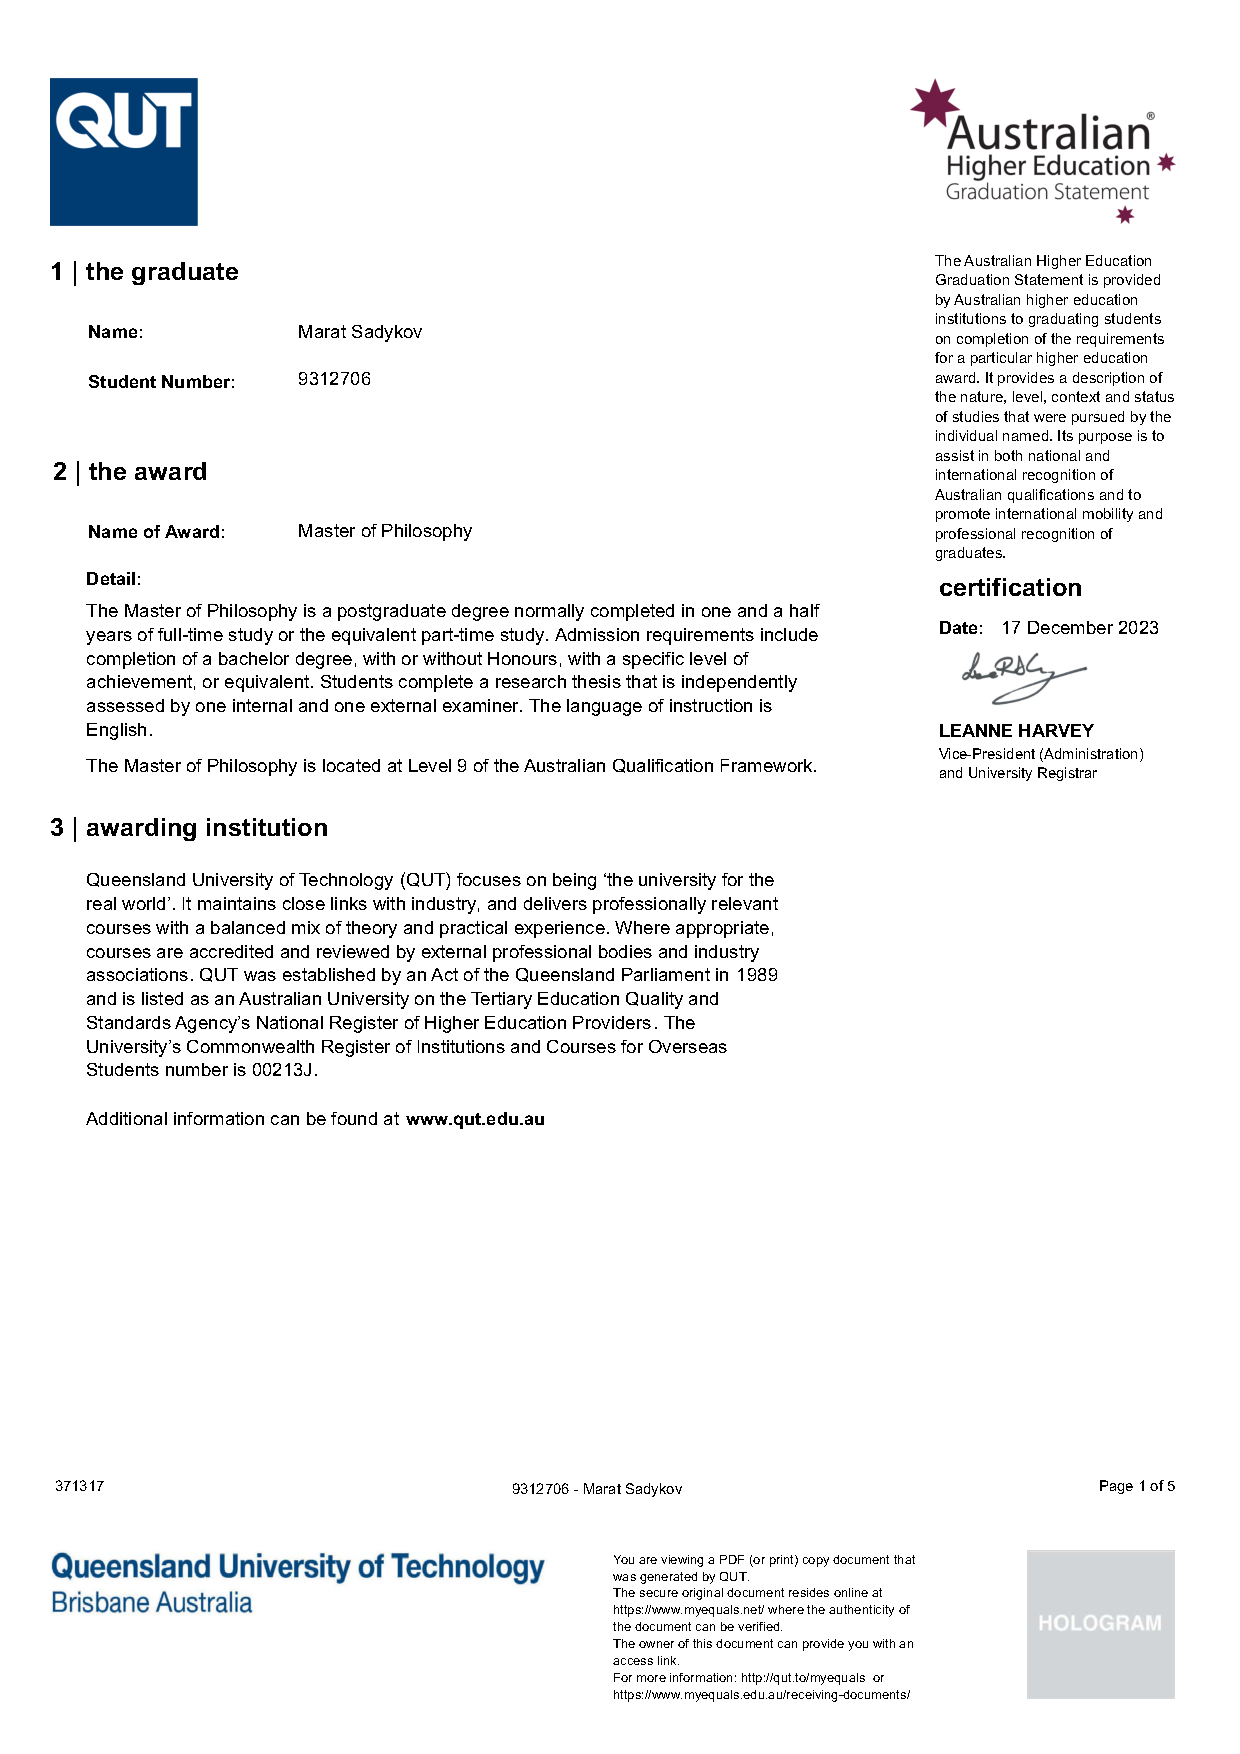
\includepdf[pages=-]{MPhil-AHEGS.pdf}
\label{bachelor}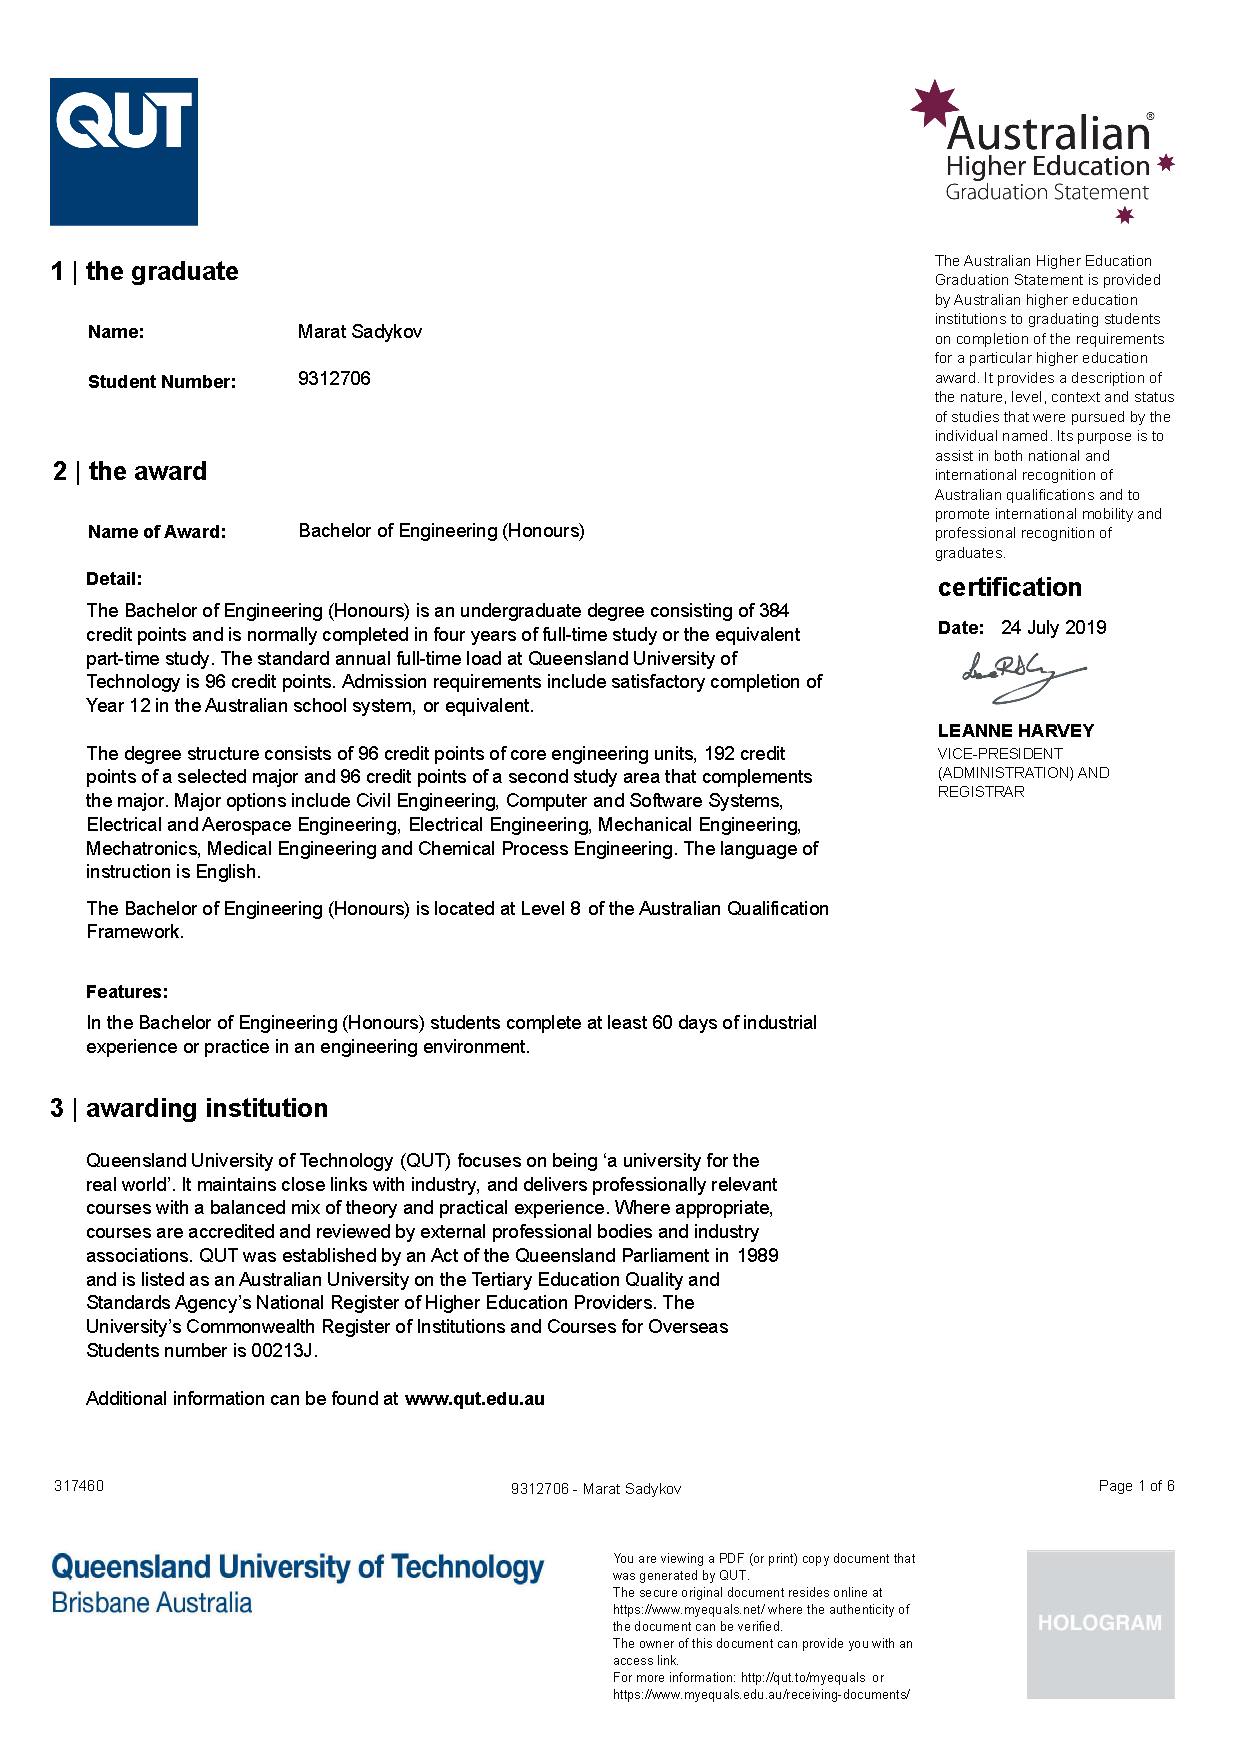
\includepdf[pages=-]{BachelorGraduationStatement.pdf}
}{}
% \XeTeXpdffile ''BachelorGraduationStatement.pdf'' page 2 scaled 800
\end{document}
